%%% Presentation slides
\newcommand{\slidesfinal}{
  \documentclass[handout,style=authortitle]{beamer}
}

%%% Ignore images --- slightly faster compilation
\newcommand{\slidestest}{
  \documentclass[demo,handout,style=authortitle]{beamer}
}

%%% Printable slides with side notes thing
\newcommand{\makehandouts}{
  \usepackage{handoutWithNotes}
  \usepackage{pgfpages}
  \pgfpagesuselayout{3 on 1 with notes big}[a4paper,border shrink=7mm]
  \pgfpageslogicalpageoptions{1}{border code=\pgfusepath{stroke}}
  \pgfpageslogicalpageoptions{2}{border code=\pgfusepath{stroke}}
  \pgfpageslogicalpageoptions{3}{border code=\pgfusepath{stroke}}
}
\slidesfinal
% \slidestest
% \makehandouts

%%% Styles and settings
\usepackage{amsmath}
\usepackage{mathtools}
\usepackage{beamerthemesplit}
\usepackage{fancybox}
\usepackage{hyperref}
\usepackage{color}
\usepackage{listings}
\usepackage{caption}
\usepackage{subcaption}


\makeatletter
\newcommand\code{\bgroup\@makeother\_\@makeother\~\@makeother\$\@codex}
\def\@codex#1{{\normalfont\ttfamily\hyphenchar\font=-1 #1}\egroup}
\makeatother

\newcommand{\bX}{\boldsymbol{X}}
\newcommand{\bx}{\boldsymbol{x}}
\newcommand{\by}{\boldsymbol{y}}
\newcommand{\bbeta}{\boldsymbol{\beta}}
\newcommand{\bepsilon}{\boldsymbol{\epsilon}}
\newcommand{\bs}[1]{\boldsymbol{#1}}


\definecolor{gray}{rgb}{.6,.6,.6}
\definecolor{orange}{rgb}{1,0.5,0}
\definecolor{grayish}{rgb}{.775, .775, .775}
\definecolor{dkgray}{rgb}{.375, .375, .375}
\definecolor{dkgreen}{rgb}{0,0.6,0}
\definecolor{mauve}{rgb}{0.58,0,0.82}
\definecolor{dkblue}{rgb}{0, 0, .5}


\setbeamercolor{alerted text}{fg=blue}


\definecolor{g11}{rgb}{0, 0, 1}
\definecolor{g12}{rgb}{0, .4, 1}
\definecolor{g13}{rgb}{0, .8, 1}

\definecolor{g21}{rgb}{0, .5, .3}
\definecolor{g22}{rgb}{.4, .5, .3}
\definecolor{g23}{rgb}{.8, .5, .3}

\lstset{ %
  language=[95]Fortran,    
  numbers=left,
  stepnumber=1,       
  numbersep=6pt,      
  showspaces=false,      
  showstringspaces=false,  
  showtabs=false,    
  frame=single,      
  rulecolor=\color{black},   
  tabsize=4,     
  captionpos=t,     
  breaklines=true,     
  breakatwhitespace=true,   
  title=\lstname,              
  basicstyle=\ttfamily\color{black}\scriptsize, 
  backgroundcolor=\color{grayish},  
  numberstyle=\tiny\color{black},  
  keywordstyle=\color{blue}, 
  commentstyle=\color{dkgreen}, 
  stringstyle=\color{mauve}, 
  xleftmargin=.1in,
  xrightmargin=.1in,
  aboveskip=0cm,
  belowskip=.2cm
}

% \lstdefinelanguage{shl}{
%   language=sh,
%   backgroundcolor=\color{black},
%   basicstyle=\scriptsize\ttfamily\color{white},
%   keywordstyle=\color{blue},
%   commentstyle=\color{dkgreen},
%   stringstyle=\color{mauve},
%   numbers=none
% }
\lstdefinelanguage{shl}{
  language=sh,
  backgroundcolor=\color{white},
  basicstyle=\scriptsize\ttfamily\color{black},
  keywordstyle=\color{blue},
  commentstyle=\color{dkgreen},
  stringstyle=\color{mauve},
  numbers=none
}


\definecolor{pbdgrn}{HTML}{005700}
\definecolor{pbdrd}{HTML}{ab0000}
\definecolor{pbdylw}{HTML}{ab7e00}
\definecolor{pbdblu}{HTML}{2b74ec}
\newcommand{\pbdR}{\textbf{\color{pbdgrn}{p}\color{pbdrd}{b}\color{pbdylw}{d}\color{pbdblu}{R}}}

\setbeamertemplate{navigation symbols}{} 

\hypersetup{
    linkcolor=,
    colorlinks=true,
    urlcolor=blue
}

\usetheme{Frankfurt}
% \usecolortheme{whale}
% \usetheme{Antibes}
% \setbeamertemplate{mini frames}{}


\newcommand{\fctn}[1]{\textcolor{green!50!blue}{#1}}
\newcommand{\rfor}[1]{\textcolor{yellow!50!red}{#1}}
\newcommand{\rcom}[1]{\textcolor{blue}{#1}}

\newcommand{\pkg}[1]{\textbf{#1}}

\newcommand{\startr}{\begin{minipage}{.04\textwidth}\ \ \end{minipage} \begin{minipage}{.91\textwidth}}

%
\newcommand{\shownum}{\title[\mytitlea]}{}
\newcommand{\hidenum}{\title[\mytitleb]{}}
% \expandafter\def\expandafter\insertshorttitle\expandafter{\insertshorttitle\hfill\insertframenumber\,/\,\inserttotalframenumber}
 

\newcounter{excount}
\setcounter{excount}{0}
\newcommand{\countex}{\addtocounter{excount}{1}\arabic{excount}}
\newcommand{\showex}{\arabic{excount}}





\useoutertheme{miniframes}
\makeatletter
  \beamer@compressfalse
\makeatother


% -------------------------------------------------------------------------
% Logos
% -------------------------------------------------------------------------

\definecolor{ORNL}{HTML}{008752}
\definecolor{UT}{HTML}{F77F00}
\setbeamercolor{title}{fg=white}
\setbeamercolor{frametitle}{fg=white}


\newcommand{\titlelogos}{}

\newcommand{\utpres}{
  \renewcommand*\titlelogos{\centering
\includegraphics[scale=.6]{pics/logos/logos_ut}}
  \logo{
\includegraphics[height=.34cm]{pics/logos/utk.png}}
  \setbeamercolor{structure}{fg=UT}
}

\newcommand{\ornlpres}{
  \renewcommand*\titlelogos{\centering
\includegraphics[scale=.6]{pics/logos/logos_ornl}}
  \logo{
\includegraphics[height=.34cm]{pics/logos/ornl.jpg}}
  \setbeamercolor{structure}{fg=ORNL}
}

\newcommand{\allpres}{
  \renewcommand*\titlelogos{\centering
\includegraphics[scale=.6]{pics/logos/logos_all}}
  \logo{\begin{tabular}{r}
\includegraphics[height=.34cm]{pics/logos/utk.png} \\ 
\includegraphics[height=.34cm]{../common/pics/logos/ornl.jpg}\end{tabular}}
  \setbeamercolor{structure}{fg=UT}
}



% -------------------------------------------------------------------------
% Subsection contents slides
% -------------------------------------------------------------------------

\newcommand{\makesubcontentsslides}{
  \hidenum
\begin{frame}[noframenumbering]
\frametitle{Contents}
 \tableofcontents[currentsection,hideothersubsections,sectionstyle=show/hide]
\end{frame}
\shownum
}
\newcommand{\tabinlist}[2]{\begin{tabular}{p{1cm}l}#1 & #2 \end{tabular}}
\newcommand{\tabinlisttwo}[2]{\begin{tabular}{p{2.8cm}l}#1 & #2 \end{tabular}}


\utpres


\newcommand{\myauthor}{Drew Schmidt}
\newcommand{\myurl}{}
\newcommand{\myfulltitle}{Introduction to Fortran }
\newcommand{\myabbrvtitle}{Introduction to Fortran }
\newcommand{\mydate}{January 16, 2014}



% Don't touch
\title{\myfulltitle}
\newcommand{\mytitlea}{\makebox[.45\paperwidth]{\myabbrvtitle\hfill%
       \insertframenumber/\inserttotalframenumber}}
\newcommand{\mytitleb}{\myabbrvtitle}
\date{\mydate \\[1.4cm] \titlelogos} 
\newcommand{\theauthorgoeshere}{\makebox[.45\paperwidth]{%
  \myurl \hfill \myauthor}}
\author[\theauthorgoeshere]{Drew Schmidt}


%%%%%%%%%%%%%%%%%%%%%%%%%%%%%%%%
\begin{document}

%%%%%%%%%%%%%%%%%%%%%%%%%%%%%%%%%%%%%%%%
%%     Title and ToC
%%%%%%%%%%%%%%%%%%%%%%%%%%%%%%%%%%%%%%%%
% titlepage
\frame{  \maketitle   }

\begin{frame}[noframenumbering,shrink]
\frametitle{Contents}
\small
\tableofcontents[hideallsubsections]
\end{frame}

\setcounter{framenumber}{0}


\section{Introduction}
\makesubcontentsslides


\subsection{Background}

\begin{frame}
  \begin{block}{What is Fortran?}\pause
  \begin{itemize}
    \item \textbf{For}mula \textbf{tran}slation system.
    \item General purpose programming language.
    \item Well-suited for mathematics and engineering.
    \item Compiled (rather than interpreted)
    \item Portable.
  \end{itemize}
  \end{block}
\end{frame}

\begin{frame}
  \begin{block}{History}\pause
  \begin{itemize}
    \item Created at IBM in 1954 as an alternative to assembly language.
    \item Debuted in the days of punch cards.
    \item Regularly gets updated to a new standard.
  \end{itemize}
  \end{block}
\end{frame}

\begin{frame}[fragile]
\begin{block}{What people think Fortran is like}
\begin{minipage}{.475\textwidth}
\begin{lstlisting}
 1121 FORMAT(I4,F8.3)
 3298 CONTINUE
      IF(MOD(I,A)
     $.EQ.Z) THEN
      GOTO 2359
      ELSE IF(MOD(I,B)
     $.EQ.Z) THEN
      GOTO 8125
      ELSE
      WRITE (*,2930) I
      GOTO 7365
      END IF
 7235 FORMAT(A,F5.3)
 7356 CONTINUE
      I=I
     $+1
      GOTO 1249
 2930 FORMAT(I4,$)
 2359 CONTINUE
\end{lstlisting}
\end{minipage}
\begin{minipage}{.475\textwidth}
  \begin{center}
    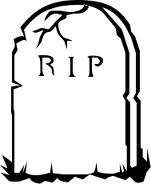
\includegraphics{pics/tombstone}
  \end{center}
\end{minipage}
\end{block}
\end{frame}


\begin{frame}
  \begin{block}{Standards}\pause
  Fortran standards are denoted by year.
  \begin{itemize}
    \item Fortran 66
    \item Fortran 77
    \item Fortran 90
    \item Fortran 95
    \item Fortran 2003
    \item Fortran 2008
    \item Fortran 2015
  \end{itemize}
  \end{block}
\end{frame}


\begin{frame}
  \begin{block}{Language Features}\pause
  Fortran essentially has two formats:  Fortran 77 and ``modern''.\\
  All versions have:
  \begin{itemize}
    \item Matrices.
    \item Complex numbers.
    \item Good interoperability with C.
    \item REALLY good compilers.
  \end{itemize}
  Modern variants of Fortran additionally have:
  \begin{itemize}
    \item Dynamic memory allocation.
    \item Pointers.
    \item OOP.
  \end{itemize}
  \end{block}
\end{frame}

\begin{frame}
  \begin{block}{Applications for Fortran}\pause
  \begin{minipage}{.475\textwidth}
  Bad applications:
    \begin{itemize}
      \item A website
      \item An OS kernel
      \item Text processing
      \item Random number generators
    \end{itemize}
  \end{minipage}
  \begin{minipage}{.475\textwidth}
  Good applications:
    \begin{itemize}
      \item Mathematics
      \item Engineering
      \item Statistics
      \item Scientific computing
    \end{itemize}
  \end{minipage}
  \end{block}
\end{frame}

\begin{frame}
  \begin{block}{Compilers}\pause
  \begin{itemize}
    \item GNU \code{gfortran} (free)
    \item Intel \code{ifortran}
    \item Portland Group \code{pgfortran}
    \item \dots
  \end{itemize}
  \end{block}
\end{frame}


\begin{frame}
  \begin{block}{Why Fortran?}\pause
  \begin{itemize}
    \item High level language
    \item Avoids fiddly memory management like in C
    \item Fortran binaries are VERY fast
    \item Good HPC support (MPI, OpenMP, \dots)
  \end{itemize}
  \end{block}
\end{frame}



\subsection{Hello World}

\begin{frame}[fragile]
\begin{block}{Hello world example}
\begin{lstlisting}[title=hello.f]
      program helloworld
      print *, "Hello world"
      end program helloworld
\end{lstlisting}
\end{block}
\end{frame}

\begin{frame}[fragile]
\begin{block}{Hello world example}
\begin{lstlisting}[title=hello.f90]
program helloworld
    print *, "Hello world"
end program helloworld
\end{lstlisting}
\end{block}
\end{frame}

\begin{frame}
  \begin{block}{Comments}
    \begin{itemize}
      \item \code{.f} is for F77, \code{.f90} is for F90+
      \item Don't use F77.
      \item Fortran is case insensitive.
      \item \code{print} and \code{write} print/write output
      \item \code{read} reads input
    \end{itemize}
  \end{block}
\end{frame}



\section{Basics}
\makesubcontentsslides

\begin{frame}
  \begin{block}{Basic Type}\pause
  \begin{itemize}
    \item Integer
    \item Real/double
    \item Complex/double complex
    \item Logical
    \item Character
  \end{itemize}
  \end{block}
\end{frame}


\subsection{Numeric Types}

\begin{frame}
  \begin{block}{Integer}\pause
  Whole numbers.
  \begin{itemize}
    \item 1
    \item -517
    \item 0
    \item Not 1.2
    \item Not $\pi$
    \item Not 0.0
  \end{itemize}
  \end{block}
\end{frame}



\begin{frame}
  \begin{block}{Real and Double}\pause
  Floating point
  \begin{itemize}
    \item 1.1
    \item 3.14159
    \item Not 1
    \item Not $\sqrt{-1}$
  \end{itemize}
  \end{block}
\end{frame}


\begin{frame}
  \begin{block}{Basic Numeric Operations}\pause
  \begin{itemize}
    \item \tabinlist{\code{a=b}:} {assign the value of \code{b} to \code{a}}
    \item \tabinlist{\code{a+b}:}{add \code{a} and \code{b}}
    \item \tabinlist{\code{a-b}:} {subtract \code{b} from \code{a}}
    \item \tabinlist{\code{a*b}:} {multiply \code{a} and \code{b}}
    \item \tabinlist{\code{a/b}:} {divide \code{b} into \code{a}}
    \item \tabinlist{\code{a**b}:} {raise \code{a} to the power \code{b}}
  \end{itemize}
  \end{block}
\end{frame}


\begin{frame}[fragile]
  \begin{block}{Quick example}\pause
\begin{lstlisting}
program arithmetic
    integer :: a = 2, b = 3

    print *, a+b
    print *, a**b
    print *, a/b
end program
\end{lstlisting}
\begin{lstlisting}[language=shl]
           5
           8
           0
\end{lstlisting}
  \end{block}
\end{frame}



\subsection{Logical Type}

\begin{frame}
  \begin{block}{Logical}\pause
  Logical variables can take two values:
  \begin{itemize}
    \item \code{.true.}
    \item \code{.false.}
  \end{itemize}
  \end{block}
\end{frame}

\begin{frame}
  \begin{block}{Comparing Logicals}\pause
  \begin{itemize}
    \item \tabinlist{\code{.eqv.}} {tests if two logical expressions are equivalent}
    \item \tabinlist{\code{.neqv.}} {tests if two logical expressions are \emph{not} equivalent}
    \item \tabinlist{\code{.and.}} {the and operator}
    \item \tabinlist{\code{.or.}} {the or operator}
    \item \tabinlist{\code{.not.}} {the negation operator}
  \end{itemize}
  \end{block}
\end{frame}

\begin{frame}
  \begin{block}{Comparing Numerics}\pause
  \begin{itemize}
    \item \tabinlisttwo{\code{a<b} or \code{a.lt.b}:} {\code{a} less than \code{b}}
    \item \tabinlisttwo{\code{a<=b} or \code{a.le.b}:} {\code{a} less than or equal to \code{b}}
    \item \tabinlisttwo{\code{a>b} or \code{a.gt.b}:} {\code{a} greater than \code{b}}
    \item \tabinlisttwo{\code{a>=b} or \code{a.ge.b}:} {\code{a} greater than or equal to \code{b}}
    \item \tabinlisttwo{\code{a==b} or \code{a.eq.b}:} {\code{a} equal to \code{b}}
    \item \tabinlisttwo{\code{a/=b} or \code{a.ne.b}:} {\code{a} not equal to \code{b}}
  \end{itemize}
  The type of a numeric comparison is of type \code{logical}.
  \end{block}
\end{frame}

\begin{frame}
  \begin{block}{Comparing Numerics}\pause
  Note: The output of a comparison of numerics is logical:
  \begin{itemize}
    \item \code{a < b < c} makes no sense (types mismatch)
    \item Instead: \code{a < b .and. b < c}
  \end{itemize}
  \end{block}
\end{frame}

\begin{frame}[fragile]
  \begin{block}{Quick example}\pause
\begin{lstlisting}
program logicals
    integer :: a = 2, b = 3, c = 1

    print *, a < b
    print *, a /= b .and. a < c
end program
\end{lstlisting}
\begin{lstlisting}[language=shl]
 T
 F
\end{lstlisting}
  \end{block}
\end{frame}

\begin{frame}
  \begin{block}{Implicit Declaration}\pause
  \begin{itemize}
    \item In Fortran, variables may be used \emph{implicitly}.
    \item Do not get into the habit of doing this.
    \item You can turn this off in a program (function, subroutine) by declaring \code{implicit none}.
    \item Declaring \code{implicit none} is generally recommended.
  \end{itemize}
  \end{block}
\end{frame}

\begin{frame}[fragile]
  \begin{block}{Implicit variables quick example}\pause
Compiles:
\vspace*{-.4cm}
\begin{lstlisting}
program implicit_declaration
    a = 2
    b = 3
    print *, a+b
end program
\end{lstlisting}
Fails to compile:
\vspace*{-.4cm}
\begin{lstlisting}
program implicit_declaration
    implicit none
    a = 2
    b = 3
    print *, a+b
end program
\end{lstlisting}
  \end{block}
\end{frame}


\begin{frame}
  \begin{block}{Example}\pause
    Go to example.\\[.4cm]
    Not covered: 
    \begin{itemize}
      \item complex
      \item character
      \item kind/precision
    \end{itemize}
  \end{block}
\end{frame}

% \begin{frame}[fragile]
%   \begin{block}{Logical}\pause
% \begin{lstlisting}[language=ft]
% 
% \end{lstlisting}
%   \end{block}
% \end{frame}


\section{Control}
\makesubcontentsslides

\subsection{if-then-else}

\begin{frame}[fragile]
  \begin{block}{\code{if-then-else}}\pause
Conditionals can take a few different forms:
\begin{lstlisting}
if (condition) one-liner
\end{lstlisting}
\begin{lstlisting}
if (condition 1) then
    statement
else if (condition 2) then
    statement
else if (...) then
    ...
else
     statement
end if
\end{lstlisting}
Note: the \code{else if} and \code{else} pieces are optional
  \end{block}
\end{frame}

\begin{frame}[fragile]
  \begin{block}{\code{if-then-else} quick example}\pause
\begin{lstlisting}
integer :: score
character(len=1) :: grade

if (score < 60) then
    grade = "F"
else if (score < 70) then
    grade = "D"
else if (score < 80) then
    grade = "C"
else if (score < 90) then
    grade = "B"
else
    grade = "A"
end if
\end{lstlisting}
  \end{block}
\end{frame}



\subsection{Loops}

\begin{frame}[fragile]
  \begin{block}{\code{do} Loops}\pause
\begin{lstlisting}
do index = first, last, step
    ! statements
end do
\end{lstlisting}
  \begin{itemize}
    \item \code{index}, \code{first}, \code{last} are integers
    \item \code{step} is a non-zero integer
    \item \code{step} can be omitted (and in this case, the step is 1)
  \end{itemize}
  \end{block}
\end{frame}

\begin{frame}[fragile]
  \begin{block}{\code{do} loops quick example}\pause
\begin{lstlisting}
integer :: factorial, i, n

print *, "Give me a positive integer integer:"
read *, n

factorial = 1

do i = 2, n
    factorial = factorial * i
end do  

print *, n, "! = ", factorial
\end{lstlisting}
  \end{block}
\end{frame}


\begin{frame}[fragile]
  \begin{block}{\code{do} Loops}\pause
\begin{lstlisting}
do
    ! statements
end do
\end{lstlisting}
  \begin{itemize}
    \item \code{statements} are executed repeatedly
    \item To exit the loop, use \code{exit}
    \item To jump to the next iteration, use \code{cycle}
  \end{itemize}
  \end{block}
\end{frame}


\begin{frame}[fragile]
  \begin{block}{\code{do} loops quick example}\pause
\begin{lstlisting}
integer :: f, i, n

print *, "Give me an integer:"
read *, n

f = 1
i = 2
do
    if (i <= n) then
        f = f * i
        i = i + 1
    else
        exit
    end if
end do  

print *, n, "! = ", f
\end{lstlisting}
  \end{block}
\end{frame}


\begin{frame}
  \begin{block}{Example}\pause
    Go to example.\\[.4cm]
    Not covered: \code{do-while} loops
  \end{block}
\end{frame}
\section[Functions]{Functions, Intrinsics, and Subroutines}
\makesubcontentsslides



\subsection{Functions}

\begin{frame}[fragile]
  \begin{block}{Functions}\pause
\begin{lstlisting}
! Declaration
function foo(bar)
    type :: foo
    ! statements
end function

! Invocation
a = foo(b)
\end{lstlisting}
  \begin{itemize}
    \item Can take variety of inputs.
    \item Returns single output.
  \end{itemize}
  \end{block}
\end{frame}

\begin{frame}[fragile]
  \begin{block}{Functions quick example}\pause
\begin{lstlisting}
function circumference(r)
    implicit none
    real :: pi = 3.14159
    real :: r
    real :: circumference
    circumference = 2.0*pi*r
end function circumference

program circles
    real :: r = 2.0
    real :: circumference
    print *, circumference(r)
end program circles
\end{lstlisting}
\begin{lstlisting}[language=shl]
   12.5663605  
\end{lstlisting}
  \end{block}
\end{frame}


\subsection{Intrinsics}

\begin{frame}
  \begin{block}{Intrinsics}\pause
  \begin{itemize}
    \item Built-in functions.
    \item Casting.
    \item Basic math utilitis.
    \item Bit-shifting.
  \end{itemize}
  \end{block}
\end{frame}

\begin{frame}
  \begin{block}{Intrinsic Examples}\pause
  {\small
    \begin{tabular}{ll|ll}\hline
      Intrinsic & Effect & Intrinsic & Effect\\\hline
      \code{int} & Convert to \code{integer} & \code{mod} & Modular arithmetic\\
      \code{real} & Convert to \code{real} & \code{abs} & Absolute value\\
      \code{floor} & Greatest integer below & \code{sqrt} & Square root\\
      \code{ceiling} & Smallest integer above & \code{exp} & Exponential\\\hline
    \end{tabular}
  }
  \end{block}
\end{frame}

\begin{frame}[fragile]
  \begin{block}{Intrinsics quick example}\pause
\begin{lstlisting}
integer :: a = 2, b = 3

print *, mod(3, 2)
print *, real(a/b)
print *, real(a) / real(b)
 \end{lstlisting}
\begin{lstlisting}[language=shl]
           1
   0.00000000    
  0.666666687
\end{lstlisting}
  \end{block}
\end{frame}



\subsection{Subroutines}

\begin{frame}[fragile]
  \begin{block}{Subroutines}\pause
\begin{lstlisting}
! Declaration
subroutine foo(bar, baz)
    type :: bar, baz
    ! statements
end subroutine

! Invocation
call foo(a, b)
\end{lstlisting}
  \begin{itemize}
    \item Can take variety of inputs.
    \item Returns a variety of outputs (modifying values of inputs).
    \item Equivalent in C is \code{void} function.
  \end{itemize}
  \end{block}
\end{frame}

\begin{frame}[fragile]
  \begin{block}{Intent}\pause
  \begin{itemize}
    \item Can declare intention of use for variable.
    \item \code{intent(in)}, \code{intent(out)}, \code{intent(inout)}.
    \item Like \code{implicit none}, not strictly necessary, but useful.
  \end{itemize}
\begin{lstlisting}
subroutine foo(a, b)
    integer, intent(in) :: a
    integer, intent(out) :: b
    ! statements
end subroutine
\end{lstlisting}
  \end{block}
\end{frame}


\begin{frame}[fragile]
  \begin{block}{Subroutine quick example}\pause
\vspace*{-.4cm}
\begin{lstlisting}
subroutine circ_stuff(r, circumference, area)
    implicit none
    real :: pi = 3.14159
    real, intent(in) :: r
    real, intent(out) :: circumference, area
    circumference = 2.0 * pi * r
    area = pi * r * r 
end subroutine circ_stuff

program circles
    real :: r = 2.0, circumference, area
    call circ_stuff(r, circumference, area)
    print *, "Circumference = ", circumference
    print *, "Area = ", area
end program circles
\end{lstlisting}
\vspace{-.2cm}
\begin{lstlisting}[language=shl]
 Circumference =    12.5663605    
 Area =    12.5663605   
\end{lstlisting}
  \end{block}
\end{frame}


\begin{frame}
  \begin{block}{Example}\pause
    Go to example.
  \end{block}
\end{frame}

\section{Precision}
\makesubcontentsslides


\begin{frame}
  \begin{block}{Precision}\pause
    In C, there are two floating point types
    \begin{itemize}
      \item \code{float}
      \item \code{double}
    \end{itemize}
    In elder Fortran, the corresponding types are
    \begin{itemize}
      \item \code{real}
      \item \code{double precision}
    \end{itemize}
  \end{block}
\end{frame}


\begin{frame}
  \begin{block}{Scientific Notation and Precision}\pause
\begin{align*}
\text{number} = \text{mantissa}\times 10^{\text{exponent}}\\
1.234 = 1234\times 10^{-4}
\end{align*}
    \begin{itemize}
      \item \code{real}: 23 bit of mantissa, 8 bits of exponent, and 1 sign bit.
      \item \code{double precision}: 52 bit of mantissa, 11 bits of exponent, and 1 sign bit.
    \end{itemize}
    \begin{itemize}
      \item \code{real}: $\approx$ 6 decimal digits of precision
      \item \code{double precision}: $\approx$ 15 decimal digits of precision
    \end{itemize}
  \end{block}
\end{frame}


\subsection{Kind}

\begin{frame}[fragile]
  \begin{block}{Kind}\pause
    \begin{itemize}
      \item \code{kind} is a parameter that specifies the storage/precision of a type (beyond its default)
      \item \code{real(kind=4)}
      \item Different compilers assign different meaning to \code{kind}.
      \item Avoid this complexity with the intrinsic functions \code{selected_<type>_kind}
    \end{itemize}
    \begin{itemize}
      \item \code{real(kind=selected_real_kind(6))}
      \item \code{real(kind=selected_real_kind(15))} 
      \item \dots
    \end{itemize}

  \end{block}
\end{frame}

\begin{frame}[fragile]
  \begin{block}{Quick example}\pause
\begin{lstlisting}
program kind_example
    implicit none
    integer, parameter :: r15 = selected_real_kind(15)
    real :: x
    real(kind=r15) :: y
    
    x = 1.0
    y = 1.0
    
    print *, x
    print *, y
    
end program
\end{lstlisting}
\begin{lstlisting}[language=shl]
   1.00000000    
   1.0000000000000000  
\end{lstlisting}
  \end{block}
\end{frame}


%%%%%%%%%%%%%%%%%%%%%%%%%%%%%%%%%%%%%%%%
%%     Last few slides
%%%%%%%%%%%%%%%%%%%%%%%%%%%%%%%%%%%%%%%%
\section{Wrapup}
\makesubcontentsslides



\begin{frame}
  \begin{block}{Other Important Topics Not Discussed Here}
    \begin{itemize}
      \item Debugging
      \item Arrays
      \item Pointers
      \item Interfacing to C
      \item Tabs versus spaces
    \end{itemize}
  \end{block}
\end{frame}


\begin{frame}
  \begin{block}{Some languages come and go}
    \begin{center}
      
\includegraphics[scale=.7]{pics/lifecycle}
    \end{center}
  \end{block}
\end{frame}

\begin{frame}
  \begin{block}{But with Fortran\dots}
    \begin{center}
      
\includegraphics[scale=.5]{pics/here_forever}
    \end{center}
  \end{block}
\end{frame}

\begin{frame}
  \begin{block}{Because when the USS Enterprise makes her maiden voyage}
    \begin{center}
      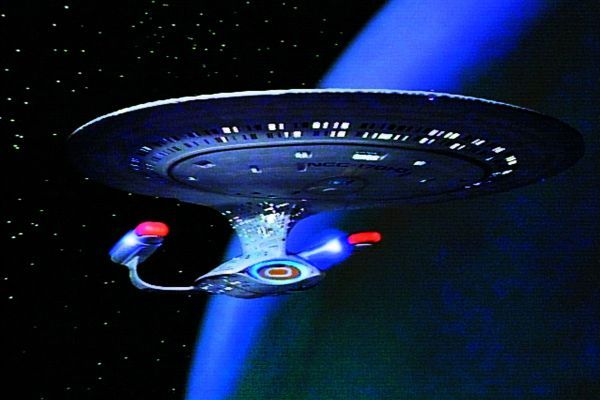
\includegraphics[scale=2]{pics/enterprise}
    \end{center}
  \end{block}
\end{frame}

\begin{frame}
  \begin{block}{Beneath the fancy blinking screens}
    \begin{center}
      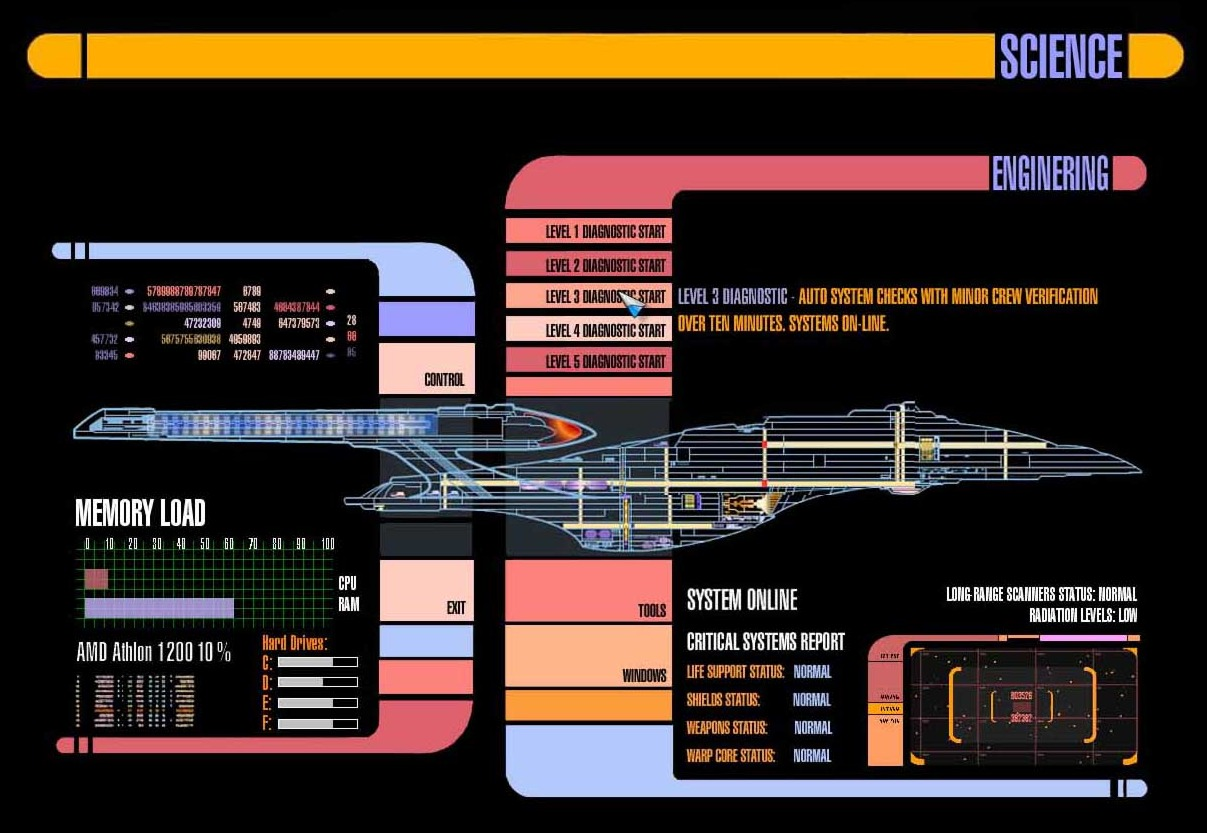
\includegraphics[scale=.33]{pics/lcars}
    \end{center}
  \end{block}
\end{frame}

\begin{frame}
  \begin{block}{You can bet that their crucial systems are powered by Fortran written in the 1970's}
    \begin{center}
      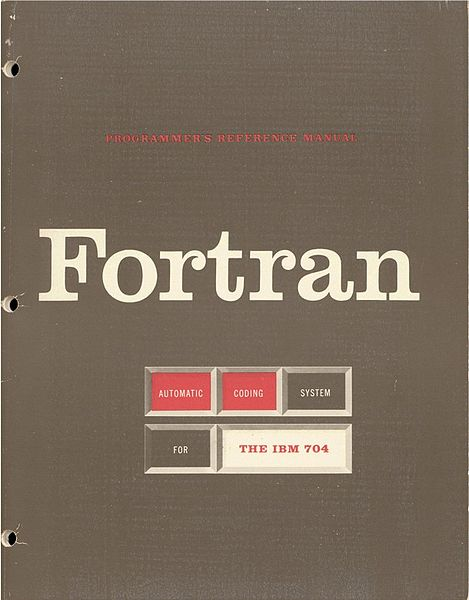
\includegraphics[scale=.3]{pics/fortran}
    \end{center}
  \end{block}
\end{frame}



\section*{}



\begin{frame}[noframenumbering]
 \begin{block}{Thanks for coming!}
 \begin{center}
 \vspace{.4cm}
     {\Huge Questions?}\\[.8cm]
  \end{center}
 \end{block}
\end{frame}



\end{document}
%%%%%%%%%%%%%%%%%%%%%%%%%%%%%%%%